
% This LaTeX was auto-generated from MATLAB code.
% To make changes, update the MATLAB code and republish this document.

\documentclass{article}
\usepackage{graphicx}
\usepackage{color}

\sloppy
\definecolor{lightgray}{gray}{0.5}
\setlength{\parindent}{0pt}

\begin{document}

    
    
\subsection*{Contents}

\begin{itemize}
\setlength{\itemsep}{-1ex}
   \item Rotary pendulum analysis and control
   \item From state space to transfer function
   \item Computing $H(s)$
   \item Verifying the two transfer functions
   \item Plant transfer functions
   \item Verifying the transfer function representation in simulink
   \item Plant step response
   \item System stability and poles
   \item Feedback gain vector k
   \item State space representation with full state feedback
   \item Verifying new state space representation
   \item Pendulum animation
   \item LQR method
\end{itemize}


\subsection*{Rotary pendulum analysis and control}

\begin{verbatim}
XX = 24;
YY = 08;
ZZ = 18;
g = 9.81;
L_a = (10+XX*20/100)*0.01;
L_p = (5+YY*25/100)*0.01;
M_a = L_a/10+0.04;
M_p = ZZ/100;
J_a = (M_a *L_a^2)/12 ; J_p = (M_p*L_p^2)/12 ; J_t = J_a*J_p + J_a*M_p*(L_p/2)^2 + J_p*M_p* L_a^2;
A = [0 0 1 0 ; 0 0 0 1; 0 M_p^2*L_p^2*L_a*g/(4*J_t) 0 0;0 M_p*L_p*g*(J_a+M_p*L_a^2)/(2*J_t) 0 0];
B = [0;0;(J_p + 1/4*M_p*L_p^2)/J_t ; M_p*L_p*L_a/(2*J_t)];
C = [1 0 0 0; 0 1 0 0 ];
D = [0;0];
sys_ss = ss(A,B,C,D); %state space representation
\end{verbatim}


\subsection*{From state space to transfer function}

\begin{par}
To convert our state space equations to transfer function form, we need to find $H(s)$ such that:
\end{par} \vspace{1em}
\begin{par}
$$ Y(s) = H(s)T(s) $$
\end{par} \vspace{1em}
\begin{par}
First, we take the laplace transform of both our state space equations:
\end{par} \vspace{1em}
\begin{par}
$$\mathcal{L}\left[ \dot{x}(t) \right] = \mathcal{L}\left[ Ax(t) + BT(t) \right] $$
$$ sX(s) = AX(s) + BT(s) $$
\end{par} \vspace{1em}
\begin{par}
And for our output equation:
\end{par} \vspace{1em}
\begin{par}
$$ \mathcal{L}[y(t)] = \mathcal{L}\left[ Cx(t) \right] $$
$$ Y(s) = CX(s) $$
\end{par} \vspace{1em}
\begin{par}
We can factor out and isolate $X(s)$ in our first equation:
\end{par} \vspace{1em}
\begin{par}
$$ (Is - A)X(s) = BT(s) $$
$$ (Is-A)^{-1} (Is-A)X(s) = (Is-A)^{-1}BT(s) $$
$$ X(s) = (Is-A)^{-1}BT(s) $$
\end{par} \vspace{1em}
\begin{par}
We can insert this expression for $X(s)$ into our second equation:
\end{par} \vspace{1em}
\begin{par}
$$ Y(s) = C(Is-A)^{-1}BT(s)U(s) $$
\end{par} \vspace{1em}
\begin{par}
Finally, we can divide by $U(s)$ on both sides to find our transfer function:
\end{par} \vspace{1em}
\begin{par}
$$ H(s) = \frac{Y(s)}{U(s)} = C(Is-A)^{-1} $$
\end{par} \vspace{1em}


\subsection*{Computing $H(s)$}

\begin{par}
Let's find the transfer function for our system, manually and with matlab's functionality.
\end{par} \vspace{1em}
\begin{par}
I round off the entries in A to make my life a bit easier.
\end{par} \vspace{1em}
\begin{verbatim}
A = [0 0 1 0;
     0 0 0 1;
     0 181 0 0;
     0 782 0 0;];

B = [0;
     0;
     921;
     2921;];

C = [1 0 0 0;
     0 1 0 0];

D = [0;
     0];

sys_ss = ss(A, B, C, D);
s = tf('s');
\end{verbatim}
\begin{par}
The easy way:
\end{par} \vspace{1em}
\begin{verbatim}
H_matlab = tf(sys_ss);
\end{verbatim}
\begin{par}
Manually:
\end{par} \vspace{1em}
\begin{verbatim}
I = eye(4); % 4x4 identity
H_manual = C*((I*s-A)\B);
\end{verbatim}
\begin{par}
We now have the transfer function for our plant, one computed with tf() and one manually.
\end{par} \vspace{1em}
\begin{verbatim}
H_matlab
\end{verbatim}

        \color{lightgray} \begin{verbatim}
H_matlab =
 
  From input to output...
       921 s^2 + 1.636e-12 s - 1.915e05
   1:  --------------------------------
        s^4 - 1.066e-14 s^3 - 782 s^2
 
                2921
   2:  -----------------------
       s^2 - 1.066e-14 s - 782
 
Continuous-time transfer function.

\end{verbatim} \color{black}
    \begin{verbatim}
H_manual
\end{verbatim}

        \color{lightgray} \begin{verbatim}
H_manual =
 
  From input to output...
                  921 s^2 - 1.178e-10 s - 1.915e05
   1:  ------------------------------------------------------
       s^4 - 1.495e-14 s^3 - 782 s^2 + 6.066e-13 s - 1.97e-29
 
         2921
   2:  ---------
       s^2 - 782
 
Continuous-time transfer function.

\end{verbatim} \color{black}
    

\subsection*{Verifying the two transfer functions}

\begin{par}
The two transfer functions seemed a little different so i plotted their step responses to make sure they behave the same:
\end{par} \vspace{1em}
\begin{verbatim}
subplot(2,1,1);
step(H_manual(1), 'b-')
title('Theta part, manual')
subplot(2,1,2);
step(H_matlab(1), 'r-')
title('Theta part, tf()')
\end{verbatim}

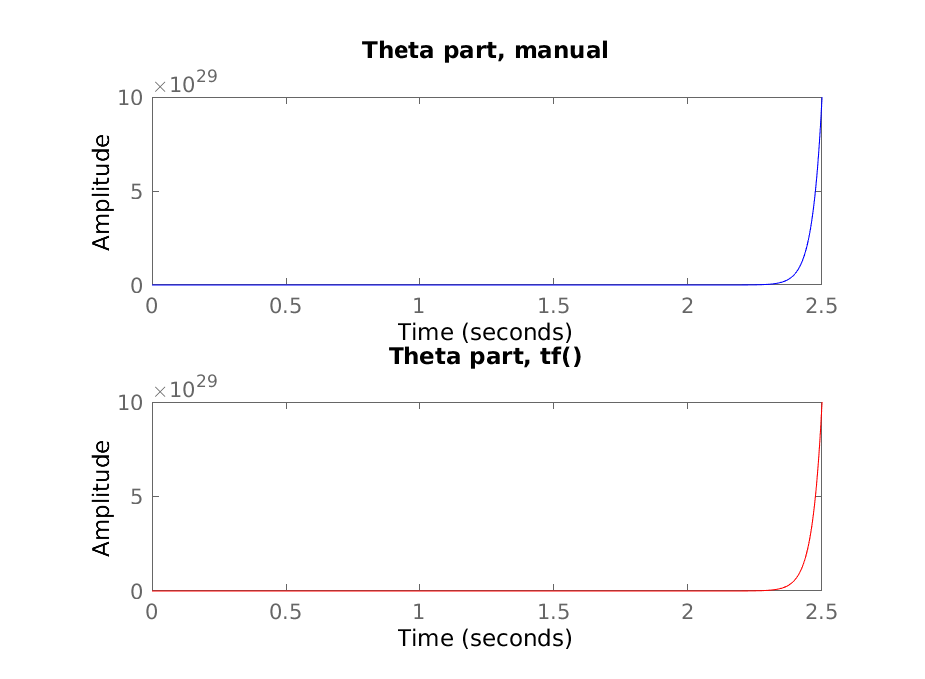
\includegraphics [width=4in]{main_01.eps}
\begin{verbatim}
close;
subplot(2,1,1);
step(H_manual(2), 'b-')
title('Alpha part, manual')
subplot(2,1,2);
step(H_matlab(2), 'r-')
title('Alpha part, tf()')
\end{verbatim}

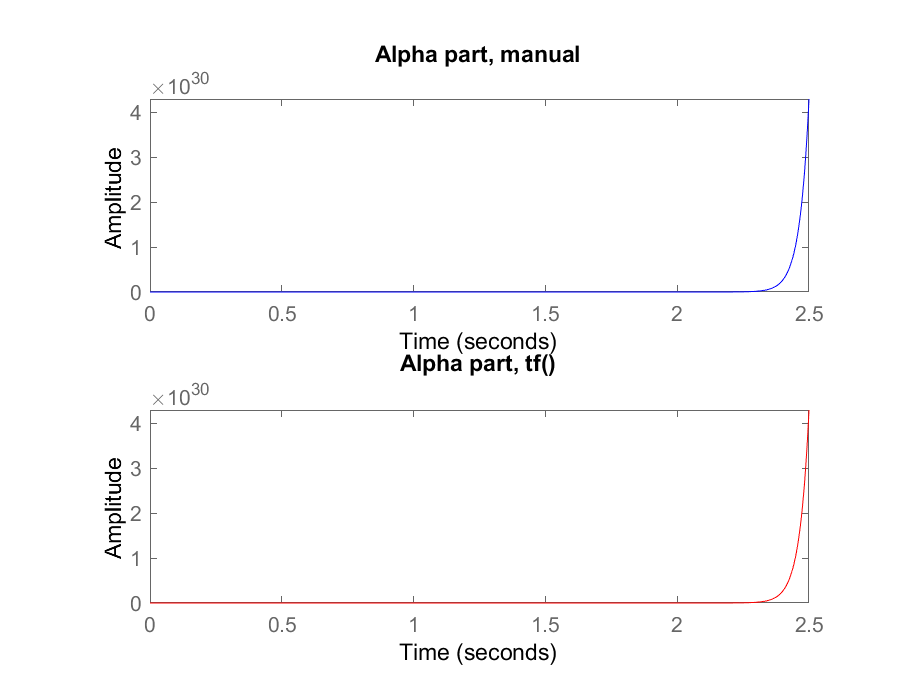
\includegraphics [width=4in]{main_02.eps}
\begin{par}
The manually computed and tf(sys\_ss) transfer functions seem to behave the same, so I conclude that they only 'look' different due to numerical differences and matlab's tf() implmentation.
\end{par} \vspace{1em}


\subsection*{Plant transfer functions}

\begin{par}
Before I move on, i remove the extremely small coefficients in the transfer functions, as they have virtually no impact) I verified this by checking that the poles didnt change.
\end{par} \vspace{1em}
\begin{verbatim}
close;

H_theta = (921*s^2 - 191500)/(s^4 - 782*s^2); %theta transfer function
H_alpha  = (2921)/(s^2-782); %alpha transfer function
H = [H_theta;H_alpha];
\end{verbatim}


\subsection*{Verifying the transfer function representation in simulink}

\begin{par}
To make sure the transfer function accurately describes our system, i plotted the responses of the original state space system together with the responses of the equivalent transfer functions.
\end{par} \vspace{1em}
\begin{par}

\includegraphics [width=4in]{ss_tf_verification_blocks.png}

\end{par} \vspace{1em}
\begin{par}

\includegraphics [width=4in]{simulink_tf_ss_verification.png}

\end{par} \vspace{1em}
\begin{par}
The responses from the two representations are identical, so we are ready to move on with the transfer function analysis. We end up with the following plant transfer functions for $\theta$ and $\alpha$:
\end{par} \vspace{1em}
\begin{par}
$$ H_{\theta} = \frac{921s^2-191500}{s^4-782s^2} $$
\end{par} \vspace{1em}
\begin{par}
$$ H_{\alpha} = \frac{2921}{s^2-782} $$
\end{par} \vspace{1em}


\subsection*{Plant step response}

\begin{verbatim}
close;
subplot(2,1,1);
step(H_theta, 'b')
title('Theta response')
subplot(2,1,2);
step(H_alpha, 'r')
title('Alpha response')
\end{verbatim}

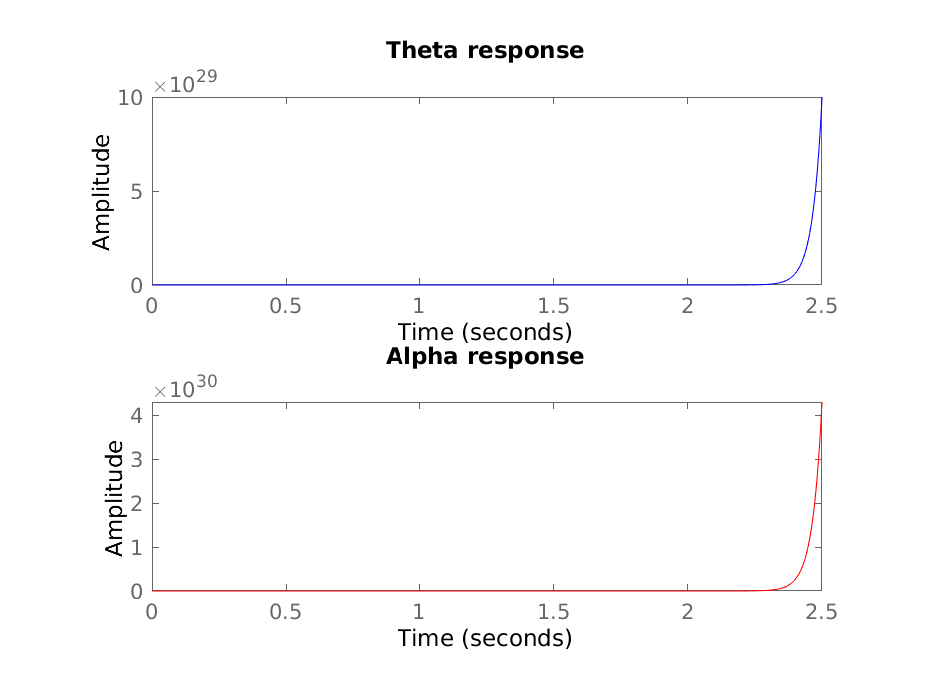
\includegraphics [width=4in]{main_03.eps}


\subsection*{System stability and poles}

\begin{par}
The system is clearly unstable in both $\theta$ and $\alpha$.
\end{par} \vspace{1em}
\begin{par}
Checking the poles with pzplot() and pole():
\end{par} \vspace{1em}
\begin{verbatim}
close;
pzplot(H);
pole(sys_ss)
\end{verbatim}

        \color{lightgray} \begin{verbatim}
ans =

         0
         0
   27.9643
  -27.9643

\end{verbatim} \color{black}
    
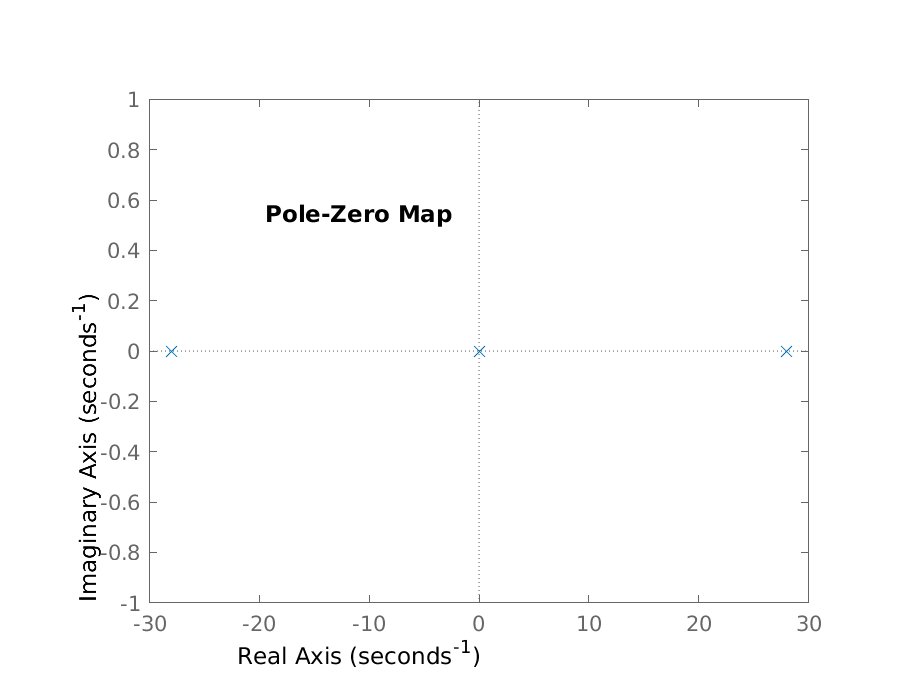
\includegraphics [width=4in]{main_04.eps}
\begin{par}
Our system has four poles:
\end{par} \vspace{1em}
\begin{par}
$$ \left[0, 0, 27.9643, -27.9643 \right]$$
\end{par} \vspace{1em}
\begin{par}
The system has poles in the right half-plane, and is therefore unstable.
\end{par} \vspace{1em}
\begin{verbatim}
close;
\end{verbatim}


\subsection*{Feedback gain vector k}

\begin{par}
We need to find a gain vector $\vec{k} = [k_1, k_2, k_3, k_4]$ Which brings the poles/eigenvalues to -10, for our system:
\end{par} \vspace{1em}
\begin{par}
$$\dot{\vec{x}} = A\vec{x} + \vec{B}T$$
\end{par} \vspace{1em}
\begin{par}
We can do this by using the acker() commands, specifying our desired pole locations
\end{par} \vspace{1em}
\begin{verbatim}
P = [-10, -10, -10, -10];
K = acker(A, B, P);
A_CL = A-B*K;
\end{verbatim}
\begin{par}
Plotting the new step response of our controlled system with desired pole placement (top: $\theta$, bottom: $\alpha$):
\end{par} \vspace{1em}
\begin{verbatim}
sim_time = 3;
new_sys = ss(A_CL, B, C, D);
\end{verbatim}
\begin{verbatim}
close;
step(new_sys);
\end{verbatim}

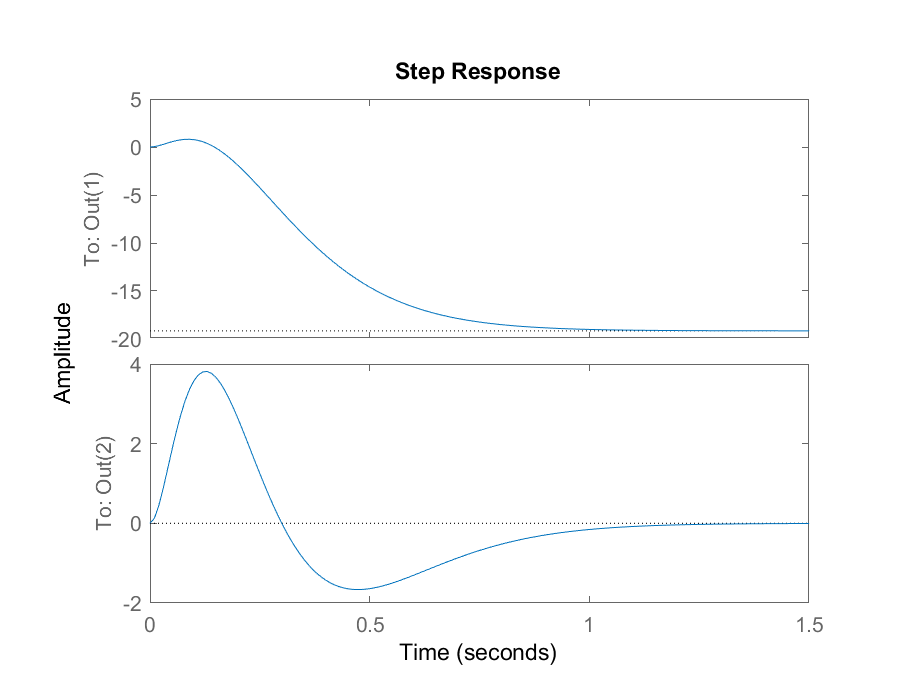
\includegraphics [width=4in]{main_05.eps}
\begin{par}
As we can see, by using full state feedback to place our poles, the system is now stable.
\end{par} \vspace{1em}


\subsection*{State space representation with full state feedback}

\begin{par}
We have found a K matrix/vector such that the poles of our new system is stable (this requires full state estimation). We did this by implicitly defining our control input $T$ as: $$ T = r-\vec{k}\vec{x} $$
\end{par} \vspace{1em}
\begin{par}
Where $r$ is the reference/input. In this way, our new system becomes:
\end{par} \vspace{1em}
\begin{par}
$$ \dot{\vec{x}} = A\vec{x} + B(r-\vec{k}\vec{x}) $$
\end{par} \vspace{1em}
\begin{par}
$$ \dot{\vec{x}} = A\vec{x} + Br-B\vec{k}\vec{x} $$
\end{par} \vspace{1em}
\begin{par}
$$ \dot{\vec{x}} = (A-B\vec{k})\vec{x} + Br $$
\end{par} \vspace{1em}
\begin{par}
We now arrive at a new state space representation of our system, by defining our modified A-matrix $A_{CL}$:
\end{par} \vspace{1em}
\begin{par}
$$ A_{CL} = (A-B\vec{k})$$
\end{par} \vspace{1em}
\begin{par}
$$ \dot{\vec{x}} = A_{CL}\vec{x} + Br $$
\end{par} \vspace{1em}
\begin{par}
$$ \vec{y} = C\vec{x} $$
\end{par} \vspace{1em}
\begin{verbatim}
A_CL
\end{verbatim}

        \color{lightgray} \begin{verbatim}
A_CL =

         0         0    1.0000         0
         0         0         0    1.0000
   48.0887 -269.9112   19.2355  -18.6771
  152.5159 -648.0887   61.0064  -59.2355

\end{verbatim} \color{black}
    

\subsection*{Verifying new state space representation}

\begin{par}
To verify that our reduced state space formulation is correct, i compare the responses in simulink:
\end{par} \vspace{1em}
\begin{par}

\includegraphics [width=4in]{new_ss_blocks_verify.png}

\end{par} \vspace{1em}
\begin{par}

\includegraphics [width=4in]{new_ss_response_verify}

\end{par} \vspace{1em}
\begin{par}
As we can see, the reduced system is identical to the original full-state feedback system.
\end{par} \vspace{1em}


\subsection*{Pendulum animation}

\begin{par}
Here I make an attempt at animating the step response of the controlled pendulum.
\end{par} \vspace{1em}
\begin{verbatim}
close;
[y, t] = step(new_sys, sim_time);
timesteps = size(t);
delta_t = sim_time/timesteps(1);

for k=1:length(t)
    draw_pendulum(y(k,:));
    %pause(delta_t);
end
\end{verbatim}

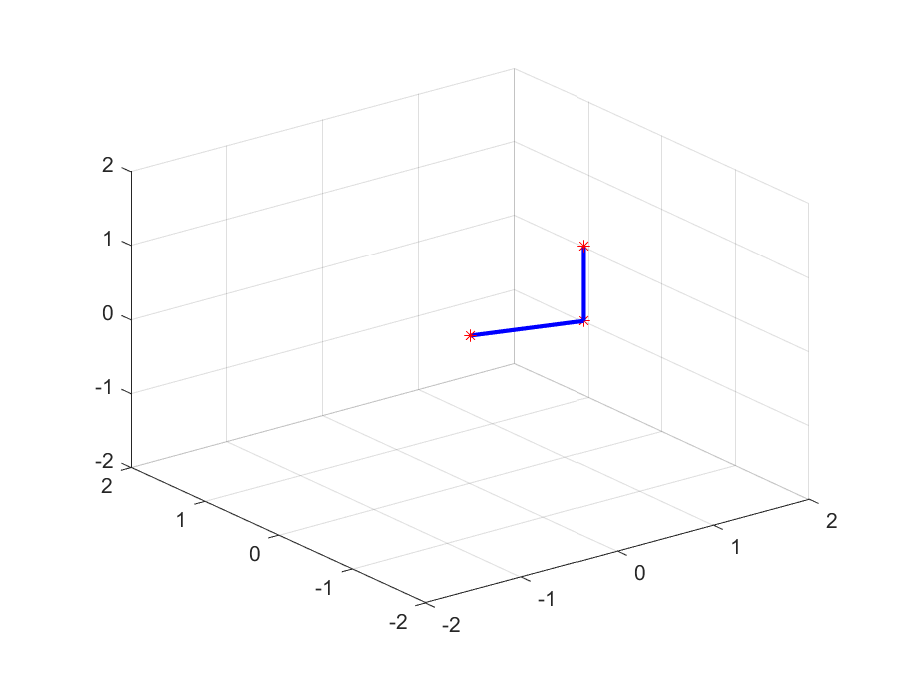
\includegraphics [width=4in]{main_06.eps}


\subsection*{LQR method}

\begin{par}
We can compute other K-vectors by defining Q and R matrices, which weight the cost of state errors and control inputs. LQR is a method of finding optimal gain matrices by minimizing the quadratic cost function:
\end{par} \vspace{1em}
\begin{par}
$$\int_0^{\infty} (x^TQx + u^TRu) dt$$
\end{par} \vspace{1em}
\begin{par}
This is a quadratic cost function, and the minima of this function has an explicit solution $\vec{u} = -K\vec{x}$. We can use the matlab lqr() function to get this gain matrix $K$, for our given system of linear ODE's and our two weight matrices $Q$ and $R$.
\end{par} \vspace{1em}
\begin{par}
In this section, i play around with different weight matrices, and see how their corresponding K-matrices affect the system. LQR assumes full-state feedback, and is similar to pole placement, except instead of specifying specific poles, we specify whether we care more about the fast convergence of certain system states, or if we care more about having a power-efficient/gentle controller.
\end{par} \vspace{1em}
\begin{verbatim}
close;
sim_time = 3;
% Doesn't care about state, terrible control:
Q = 0.0001*eye(4);
R = 10;
K = lqr(sys_ss, Q, R);
A_CL = A-B*K;
sys_lqr1 = ss(A_CL, B, C, D);
[y_lqr1, t] = step(10*sys_lqr1, sim_time);


% Aggressive controller
Q = 10000*eye(4);
R = 10;
K = lqr(sys_ss, Q, R);
A_CL = A-B*K;
sys_lqr2 = ss(A_CL, B, C, D);
[y_lqr2, t] = step(10*sys_lqr2, sim_time);

% Somewhere in between:
Q = 100*eye(4);
R = 10;
K = lqr(sys_ss, Q, R);
A_CL = A-B*K;
sys_lqr3 = ss(A_CL, B, C, D);
[y_lqr3, t] = step(10*sys_lqr3, sim_time);

% Lazy/economical controller:
Q = 10*eye(4);
R = 100;
K = lqr(sys_ss, Q, R);
A_CL = A-B*K;
sys_lqr4 = ss(A_CL, B, C, D);
[y_lqr4, t] = step(10*sys_lqr4, sim_time);


timesteps = size(t);
delta_t = sim_time/timesteps(1);
for k=1:length(t)
    draw_pendulum_2x2(y_lqr1(k,:), 1);
    draw_pendulum_2x2(y_lqr2(k,:), 2);
    draw_pendulum_2x2(y_lqr3(k,:), 3);
    draw_pendulum_2x2(y_lqr4(k,:), 4);
    %pause(delta_t);
end
\end{verbatim}

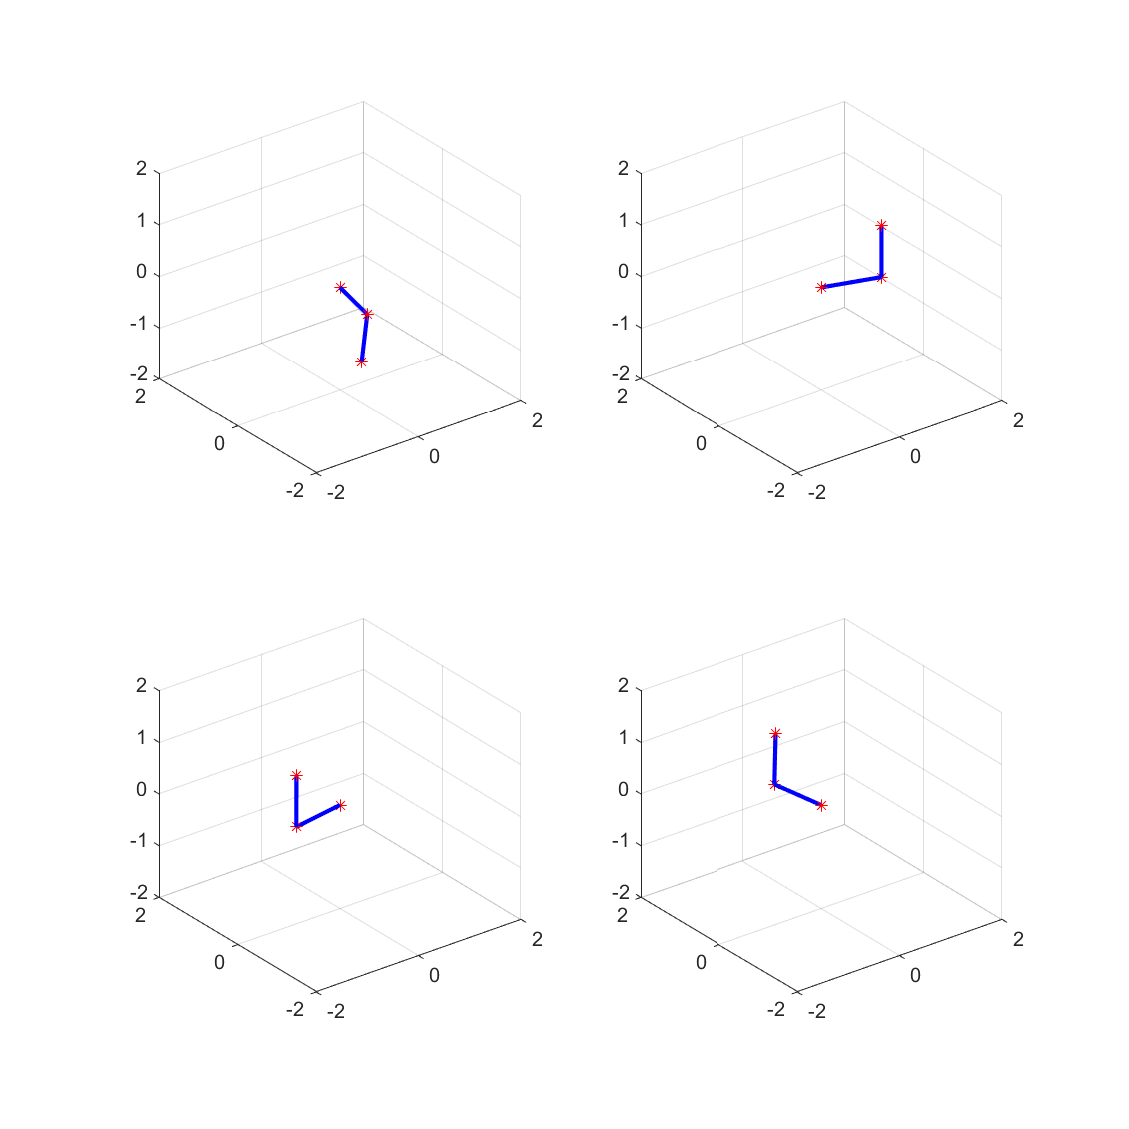
\includegraphics [width=4in]{main_07.eps}



\end{document}

